\subsection{Reactive Programming}
Reactive Programmierung wurde in den letzten Jahren immer mehr zum Trend\cite{Bainomugisha2013}. Reactive Programmierung ist ein Programmierstil, der vor allem in event gesteuerten und interaktive Anwendungen gut genutzt wird. Bekannte Unternehmen wie Amazon\footnote{https://www.amazon.de/p/feature/j5d6uh4r8uhg8ep} und Netflix\footnote{https://help.netflix.com/de/node/68708} benutzen bereits reaktive Programmierung. Dabei werden Zustands\"anderungen f\"ur das System bekannt gemacht. Wenn zum Beispiel eine Funktion aufgerufen wird, die zwei Zahlen addiert, w\"urde in dem \"ublichem Programmierstil (\textit{imperativ}) die Funktion die Variable der Summe \"andern. Wenn nach der Ausf\"uhrung der Funktion die Variablen sich \"andern w\"urden, h\"atte das keinerlei Auswirkungen auf die Summenvariable. Bei einem reaktiven Programmierstil nimmt die Summenvariable den aktuellen Wert der beiden addierten Variablen an\cite{Lambert2016}. \par\medskip 
Reactive Programming ist ein Teil aus objektorientierter und ein Teil aus funktionaler Programmierung, das asynchrone und immutable Streams von Events beinhaltet. Die Streams werden miteinander kombiniert und werden von \texttt{Observables} \enquote{abgeh\"ort}. 
%TODO besser erklären
%Bei einer \"ublichen Iteration k\"onnen jederzeit die Elemente, beispielsweise einer Liste ausgelesen werden, dabei wird der Zustand(engl \enquote{state}) des Objektes preisgegeben (\textit{pull}). ???Im n\"achsten Schritt werden die \texttt{Observables} an die Daten registriert und kann die Ver\"anderung der Daten an den \texttt{Subscriber} \textit{pushen}, somit kann das Programm ohne Zustand eines Objektes auskommen und die Ver\"anderung aktualisieren\cite{Lohmuller2016}???. Dies geschieht \"uber die Operationen \texttt{map, filter} und \texttt{skip}\cite{Lee2016}.
%Wenn somit ein \texttt{Pull} ausgef\"uhrt wird, darf der Nutzer entscheiden, wann er die Daten vom Erzeuger(engl. \textit{Producer}) bekommt. Das ist in die \"ublichen JavaScript Funktionen integriert. Beim \texttt{Push}, das die  \texttt{Obersvables} nutzen, ist dies genau anders herum. Der Nutzer wei\ss{} in diesem Fall nicht, wann er die Daten bekommt. In JavaScript w\"aren es \texttt{Promises}, welche die  \texttt{Push} Funktion nutzen. Ein  \texttt{Promise} gibt den Wert zur\"uck, sobald er die Daten empfangen hat\cite{Gruijs2017}.\\
Jedoch muss bei den \texttt{Observable} zwischen \texttt{Hot} und  \texttt{Cold Observables} unterschieden werden.
Cold \texttt{Observables} sind mit Listen vergleichbar, da wie gewohnt bei der Erzeugung die Gr\"o\ss{}e fest steht und der Inhalt dementsprechend nicht ver\"andert werden kann.
Hot \texttt{Observables} sind das genaue Gegenteil, hierbei ist nicht bekannt, wie der Inhalt aussehen k\"onnte oder wie gro\ss{} das Objekt wird. Hierbei wird ein Zeitintervall erstellt, welches innerhalb der angegebenen Zeit ein Event sendet, an das sich das Objekt abbonieren (engl. \textit{subscriben}) und somit Ver\"anderungen der Daten registrieren kann.\cite{Lohmuller2016}. Diese ganze Verarbeitung l\"auft in der reaktiven Programmierung asynchon ab und macht die Programme effizienter. Bei einer asynchronen Verarbeitung wird im Gegensatz zur synchronen Verarbeitung nicht gewartet , bis das Ergebnis einer Methode zur\"uck gegeben wird, sondern l\"auft im Code weiter. Das Ergebnis wird sobald es vorhanden ist zur\"uck gegeben.

\subsection*{Reaktives System}
Um Anforderungen, Ziele und den Aufbau eines Reaktives System zu definieren, wird ein Manifest ben\"otigt. Beim Reactive Programmingwird dies als \enquote{\textit{Reactive Manifesto}} bezeichnet\cite{ReaktiveManifest2014}.
Oftmals werden reaktive Systeme als schneller und robuster bezeichnet, dass sich mit den vier Eigenschaften beschreiben l\"asst:
\begin{itemize}
\item \textbf{Responsive:} Die Antwortbereitschaft des Systems und die Erkennung von Bugs erfolgt unmittelbar\cite{Lohmuller2016}. Die Fehler k\"onnen jedoch nur durch Abwesenheit einer Antwort erkannt werden, au\ss{}erdem sollten hierf\"ur die Zeit bis zur erwarteten Antwort eingegeben werden\cite{ReaktiveManifest2014}.

\item \textbf{Resilient:} Die Widerstandsf\"ahigkeit des Systems wird bewiesen durch die immer noch vorhandene Antwortbereitschaft w\"ahrend eines Systemfehlers oder von Ausf\"allen der Hard- oder Software. Erreicht werden kann dies durch Isolation von Komponenten, Eind\"ammung von Fehlern, Replikation von Funktionalit\"atem und das Delegieren der Verantwortungen\cite{ReaktiveManifest2014}. Anfragen warten eine bestimmten Zeit auf eine Antwort, wenn diese nicht kommt, wei\ss{} der Service Bescheid und kann ihn zeitnah behandeln\cite{Lohmuller2016}.

\item \textbf{Elastic:} Elastisch bedeutet, dass das System w\"ahrend verschiedener Lastbedingungen einen konstanten Service liefert. F\"ur die Erkennung von Ver\"anderungen und die Reaktion hierauf, muss auch hier die Replikation von Funktionalit\"aten gegeben sein. Bei erh\"ohter Last werden die Replizierungsfaktoren darauf angepasst. Dabei sollten keine Einschr\"ankungen vorhanden sein\cite{ReaktiveManifest2014}. Cloud-Dienste sind eine gute L\"osung, um die Problematik einzugrenzen und das System kosteneffektiv zu betreiben\cite{Lohmuller2016}.

\item \textbf{Message Driven:} Nachrichtenorientierte Systeme benutzen eine asynchrone Nachrichtenkommunikation. Dabei werden die Komponente, die miteinander kommunizieren, entkoppelt und isoliert. Fehler k\"onnen an andere eventuell \"ubergeordnete Komponente gesendet werden. Die Systeme lassen sich an die Nachrichten h\"angen, was die \"Uberwachung von Ver\"anderungen verinfacht\cite{Lohmuller2016}. Die Nachrichten\"uberwachung veranlasst einen \"Uberblick \"uber das Laufzeitverhalten des Systems und der \"ubermittelten Nachrichtenfl\"usse\cite{ReaktiveManifest2014}.
\end{itemize}

\begin{figure}[H] 
\centering
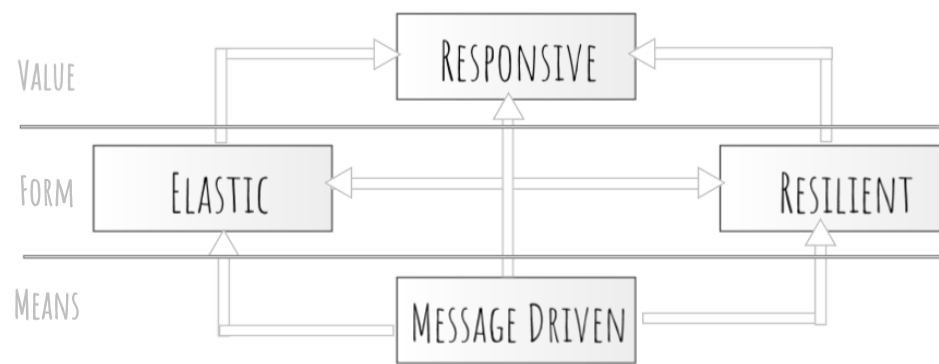
\includegraphics[scale=0.5]{fig/reaktiveSystem.png} 
\caption[Zusammenspiel reaktives System]{Zusammenspiel reaktives System \footnotemark}
\label{fig:RS}
\end{figure} 
\footnotetext{In Anlehnung an: \cite{ReaktiveManifest2014}}

In Abbildung \ref{fig:RS} wird das Zusammenspiel der vier reaktiven Qualit\"aten gezeigt.
In gr\"o\ss{}eren Anwendungen existieren mehrere Komponenten, die voneinander abh\"angig sind. Deshalb m\"ussen die vier Qualit\"aten in jeder Ebene des Gesamtsystems ber\"ucksichtigt werden und sind somit innerhalb der Schichten kombinierbar\cite{ReaktiveManifest2014}.
Frameworks helfen bei der Umsetzung eines reaktiven Programms bei den Anforderungen, Eigenschaften und Ziele. Beispiele hierf\"ur sind Vue.js und React.js.